%template taken from https://github.com/ylelkes/Internet-Speed/blob/master/Data/Crosswalks/ajps.tex

\documentclass[12pt, letterpaper]{article}

%==============Packages & Commands=================
\usepackage{graphicx} % Graphics
\usepackage{indentfirst} % Tells LaTeX to indent every paragraph 
\usepackage{setspace} % To set line spacing
\usepackage[longnamesfirst]{natbib} % For references
\usepackage{booktabs} % For tables
\usepackage{rotating} % For sideways tables/figures
\usepackage[margin = 1in]{geometry}
\usepackage{subfig}
\usepackage{mdwlist}
\usepackage{url}
\usepackage{verbatim}
\urlstyle{same}
\usepackage{multirow}
%\usepackage[nolists]{endfloat} % Figures and tables at the end. This must be commented out, along with the tableplace and figureplace commands, for tables and figs to show up in text and to compile without error. Seems to make bibpunct unrecognized too?
\bibpunct{(}{)}{;}{a}{}{,} % Reference punctuation 
\renewcommand{\cite}{\citep}
%\captionsetup[subfloat]{position = top, font = large} % For sub-figure captions

%===============Some new commands==================
\newcommand{\fnote}[1]{\footnote{\begin{doublespace}\normalsize{#1}\vspace{-26pt}\end{doublespace}}} % 12 pt, double spaced footnotes 


%============Article Title, Authors================
\title{Aiding the Enemy? Foreign Aid and Civil Conflict Intensity}
\author{Steven Saroka}

%===================Startup========================
\begin{document} 
	\maketitle
	\doublespacing
	\vspace{5.5in}
	\noindent Note: Replication data available on request from author.
	\thispagestyle{empty}
	%===================Abstract======================= 
	\newpage
	\thispagestyle{empty}
	\begin{abstract}
		\begin{normalsize}
	How does foreign aid impact conflict intensity when sent to states experiencing civil conflict? An existing body of literature describes plausible commitment problems that are theorized to occur between rebels, civilians, and the state when aid is introduced. However, the salience of these commitment problems can vary based on subnational factors, which previous studies have not always addressed. A theory of aid-related commitment problems between rebels and the state leads to predictions that aid should increase the intensity of rebel violence in urban areas, while increasing the intensity of state violence in rural areas. These hypotheses are tested for foreign aid, specifically official development assistance (ODA), at the subnational level for 27 states in Sub-Saharan Africa that experienced civil wars from 1995 through 2014. Quasi-Poisson model results fail to support these hypotheses. 
			
		\end{normalsize}
	\end{abstract}
	
	\begin{quote}
		\textbf{Keywords}: Civil war, conflict intensity, foreign aid, peace science.
	\end{quote}
	%================Begin Manuscript==================
	\newpage
\section{Introduction}
	
How does foreign aid impact conflict intensity at a regional level within states experiencing civil conflict? A substantial literature has attempted to address the question of aid’s impact on civil conflict, generating competing theories regarding the impact of foreign aid on civil conflict onset, processes, and recurrence. In particular, one strand of the literature has attempted to answer this question by focusing on the ways in which foreign aid can create commitment problems for conflict actors within the recipient state. However, competing results within this literature make clear the need for a theory of foreign aid’s impact on civil conflict processes that can account for differing regional dynamics at the subnational level.

This paper seeks to shed additional light on this topic by focusing on the theorized linkage of foreign aid to civil conflict intensity through commitment problems. Theoretically, an inflow of foreign aid into a state experiencing civil war would be expected to exacerbate the intensity of that conflict through the mechanism of a commitment problem. Foreign aid inflows threaten to upset the balance of power between the rebel group and the state, creating a shift in power that benefits one side at the expense of the other and motivating preemptive violence from whichever side will be disadvantaged by the power shift. This power shift is also expected to vary by region, creating the hypotheses that increased aid inflows will increase the intensity of rebel (state) violence in more urban (rural) areas.

While these commitment problems are theorized as occurring at the subnational level, previous efforts to investigate this topic have frequently been hampered by the lack of subnational data on aid flows. This has forced prior analyses to use the country-year as their unit of analysis, in spite of the established literature emphasizing the role of conflict processes at the subnational level. This paper provides a more direct test of these theoretical mechanisms, using subnational casualty data and geolocated foreign aid commitments for 27 states in Sub-Saharan Africa that experienced civil wars from 1995 through 2014. Testing hypotheses derived from the theory with quasi-Poisson models shows a general lack of support for them, though these null findings are qualified by some theoretical and empirical considerations.


\section{Literature Review}
\subsection{Definitions}

	Discussing the impact of aid on civil conflicts first requires a definition of “aid." Here, I adopt the definitions used in the review of the literature found in \citet{findley2018}, which define not only foreign aid but also humanitarian and strategic aid. The term “foreign aid" refers to official development assistance (ODA), which is concessional public assistance to promote economic development and welfare \cite[p.~362]{findley2018}. This contrasts with humanitarian aid, which focuses on the provision of “medical, food, and other assistance in emergency situations" (363) as well as with military aid, which is sent directly by or to a state's military. Findley also treats counterinsurgency aid as a distinct category, as this aid is "allocated by counterinsurgents directly, rather than through traditional development assistance channels" \cite[p.~363]{findley2018}. As the following review of the literature will show, studies of these distinct types of aid have developed a fairly consistent logic of aid and commitment problems. However, the implications of this logic have not been fully investigated at the subnational level, leaving a gap in the understanding of civil conflict processes.

\subsection{Aid and Civil Conflict Processes}

Within the existing literature on civil conflict processes, a primary focus has been on the impacts of humanitarian aid. Humanitarian aid, perversely, can have several negative effects. Most directly, it can be looted and then sold or otherwise used by rebels to support their war effort. This was the case with Hutu militants diverting and selling aid products originally intended for refugee camps following the Rwandan genocide \cite{cooley2002ngo,polman2010crisis} or the looting of aid vehicles and equipment in Liberia \cite[p.~366]{bryer1997better}. These incidents are specific examples of the dangers posed to humanitarian aid by its tangible nature, as it is arguably easier to loot distinct goods than it is to loot long-term development projects. Work focusing on humanitarian aid originating from the US has provided empirical support for a harmful relationship between food aid and conflict incidence and duration \cite{nunn2014us, chu2017robust}, though these findings are not unanimously agreed upon \cite{mary2020humanitarian, lehmann2021us, de2009}.

Other scholars have provided theoretical mechanisms for these outcomes. Some game-theoretic work has theorized that aid can also be directly looted by rebels, which may lead to increased conflict duration or may only be of "marginal importance" to rebels, especially if they have access to lootable natural resources in addition to aid \cite[p.~383]{addison2002}. From a bargaining perspective, humanitarian aid may obscure capabilities and therefore make it more difficult to find a bargaining range \cite{narang2015assisting}. According to this account, aid may provide an increase in capabilities for one or both sides, but with sufficient uncertainty over this increase that the net result is that true capabilities and strength become more uncertain. Additionally, there is evidence that rebels may view humanitarian aid as a challenge to their own authority as well as an opportunity for looting, which can motivate rebel violence against civilians \cite{wood2015doing}. Supporting this, \citet{wood2016aiding} find support for the association of humanitarian aid and increased violence between rebel and state forces in areas receiving aid, but note that this association does not appear to hold for other types of aid. Aid effectiveness may also be conditioned on whether recipient governments actually have incentives to follow donor development goals, as the presence of strategic donor interests or resource rents available to recipients may both derail aid effectiveness \cite{girod2012effective}. 

While this research has primarily focused on humanitarian aid, there is some evidence that accessible development aid, outside of the protection of state forces, may lead to more violence due to its targeting by rebels \cite{findley2011localized}. Other research shows that such negative impacts on conflict may not be confined to humanitarian or development aid: \citet{bapat2011} finds that US military aid creates a moral hazard problem, as states dependent on that aid have incentives to ensure it continues, even should this involve prolonging a conflict with terrorist groups that imposes costs on the population. In this vein, \citet{jadoon2018persuasion} also finds that US military aid decreases recipient state incentives to engage in civilian targeting, but development aid can create predation incentives that increase civilian targeting. Suggesting the importance of region-specific, subnational dynamics to these results, data from US counterinsurgency aid in Afghanistan show that aid can reduce violence, provided that pro-state forces control the area receiving the aid \cite{sexton2016aid}. Similar findings hold in the case of Iraq \cite{berman2013modest}. These studies show that the impacts of aid can differ based on subnational regional factors, such as whether pro-state forces control a region. While these studies focus specifically on counterinsurgency aid, these results imply the need for subnational studies of aid, due to the possibility that aid’s effects can differ within a recipient state.

The picture that emerges here is not an entirely optimistic one of aid’s impacts, with substantial though hardly unanimous support for its exacerbating impacts on conflict, but at the same time it is frustratingly incomplete. The frequent focus of this literature on humanitarian aid means that other types of aid remain under-studied. Given the difference in goals and methods across the multiple types of aid discussed above, this is a potentially significant gap in the scholarship and may help to explain the presence of the sometimes competing results found here. This is compounded by the relative lack of focus on subnational dynamics, with the few studies that have explored these dynamics suggesting that state-level analysis may obscure subnational regional differences in the impact of aid.

More fundamentally, this literature has not systematically tested the implications found here for commitment problems as a conflict process. A common theme here is that of aid as a lootable, fungible motivator for rebel group violence which can also impact the bargaining range between the rebels and the state. This would seem to imply that aid can impact commitment problems \cite{fearon1995rationalist} during conflict processes in predictable ways, motivating violence due to anticipated power shifts, but these theoretical mechanisms are not usually explicitly tested. This absence is made all the more puzzling by the presence of theories incorporating commitment problems in explanations of conflict onset and recurrence. 

\subsection{Conflict Onset, Recurrence, and Commitment Problems}

Foreign aid has been theorized to impact civil war onset through several distinct pathways. Early game-theoretic work posited that aid makes control of the state even more valuable, potentially motivating conflict over the state to control that aid unless state leaders used some aid proceeds to pay off their potential opponents \cite{azam1995, grossman1992}. Additional work in this vein has theorized that aid can be directly looted by rebels, creating additional incentives to initiate a conflict \cite[p.~383]{addison2002}. More recent theoretical and empirical work has argued that this positive impact on the probability of conflict is conditional on a combination of weak institutions in a recipient state, combined with a sudden positive increase in aid \cite{besley2011}. 

Notably, this theorizing contains elements that contribute to theorizing about commitment problems, conceptualizing of aid inflows as valuable and worth fighting over or looting. Nielsen argues that sudden negative changes in aid ("aid shocks") may increase rebel power relative to the government, potentially motivating civil conflict \cite{nielsen2011}. This takes the form of a commitment problem: during an aid shock, bargaining power shifts to favor the rebel group(s) at the expense of the government, which can attempt to mitigate this by promising the transfer of resources to appease the rebels. However, as neither side knows if the aid shock will be temporary, and the government will have incentives to renege on any resource-sharing agreement if the aid shock proves to be temporary, the two sides may be unable to reach any agreement, leading to violence. This risk may be mitigated as the number of donors increases \cite{gutting2017}, or by non-OECD Chinese foreign aid, which is less likely to cease due to sanctions \cite{strange2017}. Even so, volatility in aid disbursement increases conflict risk \cite{nourou2020}. These findings imply a clear direction for study: if aid creates a commitment problem contributing to conflict onset, it seems reasonable that similar problems could also occur during the conflict itself.

This scholarship is not monolithic, with some theorizing that aid can decrease the probability of civil conflict. Foreign aid has been posited to do so by stimulating economic growth and decreasing dependence on primary commodities \cite{collier2002aid, collierhoeffler2004} while also strengthening the state and thus discouraging potential rebels \cite{collier2011wars}. In the event of detrimental economic shocks, aid may provide low-income states with additional resources they can use to decrease the likelihood of civil war by making it less appealing for potential rebels \cite{savun_tirone_2012}. In the specific context of regimes that are in the process of democratization, the provision of democracy aid may increase stability and prevent civil war by helping to alleviate uncertainty and commitment problems surrounding commitments made by the government \cite{savuntirone2011}. Any such calming effect of aid, however, is qualified by the possibility of biased aid allocation at the subnational level \cite{jablonski2014}, which could fuel grievances motivating civil war should aid be distributed unevenly across rival ethnic or religious groups. Concerns over uneven aid allocation also occur in a post-conflict context, as \citet{narang2014humanitarian} argues that humanitarian aid will, if distributed according to need, will often be distributed in favor of the losing side of a civil war. This may provoke a shift in power, creating a classic commitment problem as the losing side seeks to renegotiate the settlement. Again, some of these findings suggest that aid’s effects can differ based on subnational differences, which may contribute to some of these divergent findings on the effects of aid. These divergent results may be due in part to competing subnational effects of aid, emphasizing the need for a subnational focus on the effects of aid on these commitment problems.

Regardless of the specific predictions of these theories of civil conflict onset and recurrence, the frequent use of commitment problems in this literature provides relatively clear implications for the exacerbating effects of commitment problems on ongoing civil conflicts, as well as the need for a subnational focus. The following theory section articulates these commitment problems and their implications at the subnational level.

\section{Theory}

As the literature review shows, commitment problems are a vital part of the accounts of conflict processes. Thus, they form the core of the theory of conflict intensity described in this section. This section proceeds as follows. First, it describes important scope conditions regarding the conflict timeframe and types of aid that are included in this theory. Then, it describes how aid’s benefits can accrue to state or rebel forces in an unbalanced way due through variation in who captures the initial benefits of aid, ultimately creating a commitment problem between the two sides due to shifting power. This commitment problem, combined with regional variations and shifts in aid inflows over time, ultimately leads to predictions regarding conflict intensity.

\subsection{Scope Conditions}

This theory focuses on aid provision’s impact on the intensity of civil conflicts. This means that this theory focuses on conflict processes rather than on conflict onset, as the commitment problem occurs in the context of preexisting tensions between rebels and the state. Thus, this theory begins in the context of an ongoing civil war, and does not attempt to address the question of conflict onset, though future work could indeed focus on onset. 

Importantly for the scope of this theory, not all aid is equivalent. Previous work has described aid in a variety of ways. Even a brief survey of the literature finds aid described in terms of fungibility \cite{bermeo2016}, as intended to bolster democratic regimes \cite{savuntirone2011}, as sent with conditionality \cite{carnegiemarinov2017}, and as military aid and a source of moral hazard \cite{bapat2011}. As it is clear from this that the concept of foreign aid can be conceptualized in various different ways, this means that any theory of aid must be transparent with regards to its theorization of aid. Here, I adopt relatively simple typology of foreign aid that follows widely used definitions in the literature. Namely, I divide aid into two broad categories based on its intent: security-oriented or not. Of the subset of aid that is not security-oriented, I further classify such aid as either development-oriented or humanitarian. This theory is primarily applicable to aid types that are not security-oriented, and in particular focuses on development aid.

I define security-oriented aid as any transfer of currency or technology that is clearly intended to strengthen the military or security forces of the recipient state. This includes both military aid, sent to or from a state’s military, and counterinsurgency aid, which is distributed directly by forces engaging in counterinsurgency \cite[p.~363]{findley2018}. Of the subset of foreign aid that is not security-oriented, I define humanitarian aid as aid which focuses on the provision of "medical, food, and other assistance in emergency situations" \cite[p.~363]{findley2018}. Meanwhile, foreign aid refers to official development assistance (ODA), which is concessional public assistance to promote economic development and welfare \cite[p.~362]{findley2018}. The empirical testing of this theory focuses specifically on the impacts of official development assistance (development aid), as it creates both winners and losers in the domestic context, ultimately leading to the commitment problem described in the next section. This does not exclude the possibility that similar commitment problems could be caused by other types of aid, such as security-oriented aid, which could be addressed in future research.

\subsection{Winners and Losers of Development Aid}

The introduction of foreign aid into the context of an ongoing civil conflict will have varying effects on conflict intensity due to two factors: the initial beneficiaries of aid and regional variation. These factors create the conditions for a commitment problem facing rebels and the state, which is triggered when aid inflows shift over time.

Development aid creates winners and losers. While this is true in the domestic contexts described in the literature review, this theory proposes that it is also true within the context of a state experiencing civil conflict. Should such a state experience an inflow of aid, the initial benefits of that aid will tend to accrue primarily to elites. These elites are typically in the government of the state or closely associated with it, and thus are uniquely well-positioned to capture the benefits of incoming aid flows by virtue of their control of the apparatus of government to which aid is disbursed. This contrasts with the position of most rebels, who are much less likely to enjoy such privileged access. This unbalanced accrual of the benefits of aid creates the conditions for a commitment problem.

This commitment problem involves the power relationship of the rebels with the government of the state. If foreign aid will disproportionately benefit the state directly and/or groups aligned with the state, then this implies that foreign aid will increase the capability of the government.\footnote{One potential objection to this assumption is the existence of a moral hazard problem for these state-aligned elites: if the state receives aid due to conditions that are at least partially created by the civil, and elites benefit from this aid, why would they have an incentive to encourage these offensives against the rebels if a decisive victory will imperil future aid flows? While this is possible, these elites may still be motivated to use this power to attack rebel forces. While rebel victory is unlikely \cite{fortna2015terrorists}, it still represents a meaningful threat to these elites who would risk losing their wealth and potentially lives. In risk management terms, it is an event with low risk but very high impact. Given this high potential impact, rational elites may still have an incentive to engage in violence against rebels to forestall this future.} This increase in capability can ultimately create a shift in power over time, threatening the rebel group’s efforts to seize territory and advance its goals. Should foreign aid increase the capacity of the state to the point that it can project power into areas that were previously unreachable for it, this would be a threat to the rebel group’s support base and perhaps its existence. Notably, the aid need not be explicitly security-oriented in nature for this to occur. Practically any foreign aid that increased the capacity of the state, or that freed state resources to be used elsewhere, could help the embattled state to extend its reach. One example of this is aid intended to facilitate improvements to infrastructure, such as development aid to build or improve road networks. Such aid is not military in nature, but it enables the state to both free up resources it might have otherwise spent building those roads, as well as to use them to move its troops. More generally, any aid that makes it easier for the state to project their presence into an area will disrupt the prior status quo. 

While the gains described here from development aid usually do not occur immediately, strategic rebels can still anticipate them and their likely impacts on the balance of power in the conflict. These rebels then have incentives to increase their violence in an attempt to cement their territorial gains and influence against the state, before the state grows stronger. This concern about growing state strength also explains why strategic rebels do not try to make peace, wait for aid to be disbursed, and then seize it.
 
In the unlikely event that aid does not directly increase the power of the state, but is instead captured or subverted by a rebel group, a commitment problem will still occur. If rebels are able to capture aid and translate it into increased power relative to the state, the same balance-of-power commitment problem happens but with the positions of the actors reversed. A strategic state anticipating future relative weakness against rebels, due to a shift in power from aid, will also anticipate these changes to the balance of power and have similar incentives to increase its violence in order to solidify its territorial holdings. While this scenario is less likely than the first scenario, as aid is usually disbursed to governments and is less likely to wind up in the hands of rebel elites, it still illustrates the broader issue of commitment problems due to power shifts created by aid.

	
\subsection{Regional Variation and Aid Inflow Shifts}

The commitment problem described above, and its effects on aid, should also vary by region. Some evidence of this has already been found in investigations of other types of aid. In Afghanistan, data from US counterinsurgency aid show that aid can reduce violence, conditional on pro-state forces controlling the area \cite{sexton2016aid}. Otherwise, insurgent groups will be able to violently resist \cite{sexton2016aid}. While these findings concern counterinsurgency aid, I theorize that shifts in foreign aid inflows over time may combine with this commitment problem to create changes in the intensity of the conflict. However, aid inflows can and do vary by region, creating the need for the subnational focus of the analysis presented here, as higher levels of aggregation (such as the country-year level) may conflate competing results and ultimately obscure evidence for this theory. 

This variation in positioning by region will be driven primarily by an urban/rural divide. As state forces are generally stronger closer to urban centers, while rebels are generally stronger in more rural areas \cite{kalyvas2006logic}, these differentials will influence which side is better positioned to benefit from any change in aid inflow in a given region. Additionally, this urban/rural power dynamic is easily observed by both sides of a conflict, allowing both to reasonably anticipate the impacts of aid inflows over time, and to act in anticipation of power shifts in a given region. These power shifts are triggered when aid disrupts the status quo of a region by enabling a side to expand its power into areas that were previously too costly or distant for that side to influence. In the example above of development aid for building a road network, such a network would enable state forces to more and quickly efficiently venture out from urban centers and into the countryside, making it easier for them to threaten previously safe rebel holdings. Even in cases where the aid is not so clearly focused on something directly conflict-relevant, like transportation infrastructure that enables troops to move more easily, the introduction of external resources in the form of aid still means that the side benefiting from them gains some advantage, as these inflows of aid serve to free up resources that can then be used in the conflict itself.

When aid is sent to more urban areas, the shift in power enabled by this aid will be viewed by rebels as a precursor to state forces expanding and solidifying their hold on the region. Rebels will anticipate this outcome due to their knowledge that state forces are generally stronger closer to urban centers, and so better positioned to ensure that they are able to capitalize on any incoming aid. This increased strength will then trigger the commitment problem, leading rebels to increase their violence in an attempt to secure their territorial gains. This implies a first hypothesis:

	\textbf{H1: increased aid inflows will increase the intensity of rebel violence in more urban areas.}
	
The reverse of this is expected to occur in more rural areas. In these areas, a shift in power in the form of increased aid will be viewed by the state as a precursor to the rebels gaining a stronger foothold in the region. State forces will then attempt to stop the rebels from locking in these gains, leading to an increase in conflict intensity. However, this will be violence primarily perpetrated by the state, inflicted on rebels. This expectation forms the second hypothesis:
	
\textbf{H2: increased aid inflows will increase the intensity of state violence in more rural areas.}
	
\section{Methods}

\subsection{Data Sources}

	To test this theory, I analyze time-series data covering 27 states in Sub-Saharan Africa, from 1995 through 2014.\footnote{While a larger timeframe would be preferable, this timeframe is primarily imposed by the limits of the data, especially the geolocated aid data.} This sample includes all states in the region that experienced a civil war or internationalized civil war during this time according to the UCDP’s Armed Conflict Dataset \cite{gleditsch2002armed, davies2022organized}. The states in this analysis are listed in this footnote.\footnote{The states included in this analysis are: Angola, Burundi, Cameroon, the Central African Republic, Chad, Comoros, the Democratic Republic of the Congo,  the Republic of Congo, Cote d’Ivoire, Eritrea, Ethiopia, Guinea-Bissau, Guinea, Kenya, Lesotho, Liberia, Mali, Mauritania, Mozambique, Niger, Nigeria, Rwanda, Senegal, Sierra Leone, Somalia, South Sudan, and Sudan.} I use subnational data on aid from Aiddata’s Geoquery portal, combined with data on from the World Bank’s World Development Indicators, Varieties of Democracy (V-Dem) scores, and conflict data from the UCDP \cite{goodman2019geoquery,wb2022, vdem2023, pemstein2018v, davies2022organized, sundberg2013introducing}. 

	Geoquery, a project of the Aiddata research lab, is a geospatial data collection effort that integrates several preexisting data collection efforts with accurate data on the subnational boundaries within states \cite{goodman2019geoquery}. This allows preexisting data sets with a geographic component, such as the UCDP’s Georeferenced Event Dataset \cite{davies2022organized, sundberg2013introducing}, to be mapped to first-level subnational administrative divisions. The first administrative subdivision is the first set of administrative subdivisions within the borders of a state, which are a state’s constituent provinces or analogous territorial divisions. The unit of analysis is thus the subdivision-year.
		
	To measure conflict intensity, I match to each subdivision-year the UCDP conflict death counts from version 22.1 of the UCDP’s Georeferenced Event Dataset \cite{sundberg2013introducing} that took place within that subdivision during that year.\footnote{Due to compatibility UCDP’s datasets, this means that all of these events are also events that were coded as part of the conflicts identified in the ACD. However, I do include GED events occur even during years where the conflict is coded as inactive.} This allows the creation of variables measuring the number of deaths of state forces, rebel forces, and civilians , for each subdivision-year.\footnote{To enable accurate matching, I exclude all GED instances with a where\_prec value higher than 4. Values of 4 or below indicate that the first administrative subdivision, or even more precise location data, is known for the event.} In cases where the administrative subdivisions identified in GED events could not be matched to those administrative subdivisions contained in Geoquery, those events were excluded from this analysis. This led to the exclusion of Namibia, Uganda, and most of Sudan. 
	
	To measure aid data, I use Geoquery’s geocoded values for World Bank development aid data committed to a subdivision in a given year \cite{aiddatav142}. While a focus on disbursed aid would be ideal, Geoquery’s own documentation acknowledges the difficulty of finding more specific dates than the commitment year \cite{strandow2011ucdp}. To accommodate the possibility of a significant delay between commitment and disbursement, I lag all aid by one year. This means that all variables derived from aid figures, including both primary independent variables discussed below, are lagged by one year.
	
	 The primary independent variable in the first set of models is the yearly change in the amount of lagged development aid committed to a given subdivision in a given year, as recorded in the World Bank Donor System and compiled by Aiddata \cite{aiddatav142}. This variable is coded in millions of dollars, rather than percent change, to remain comparable to other variables. It is roughly evenly distributed around 0, with values closest to 0 being the most frequently occurring, as shown in Figure \ref{fig:aidchangehist}. This variable is used, instead of a simpler amount of lagged aid committed to a subdivision in a given year, in order to better capture the changes described in the theory. As the theory focuses on shifts in aid inflows, these shifts are best operationalized by examining the changes in the context of aid commitments over time. For example, in a subdivision that experiences a constant influx of the same amount of aid each year for several years, this aid will become an accepted part of the status quo. To operationalize these static, dependable inflows as examples of aid shifts makes little descriptive sense. By contrast, measuring the amount of change in aid year-on-year more accurately captures when inflows of aid change, creating the power shifts described in the theory. 
	
	\begin{figure}
		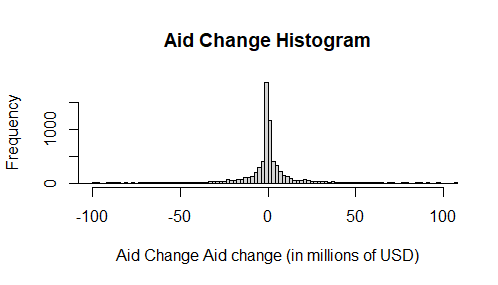
\includegraphics[scale=1]{aidchangehist}
		\caption{Histogram of Aid Change Variable. The x-axis range excludes some outlier points, but those do not affect the overall shape of the distribution}
		\label{fig:aidchangehist}
	\end{figure}
	
	Geoquery also provides subdivision population data \cite{worldpop} from 2001 onward. For the 2001 through 2014, this data can be used to weight aid change by population. This enables the creation of another primary independent variable, which is the amount of lagged aid change in millions per million residents of the subdivision. This variable is distributed very similarly to the other primary independent variable, as shown in Figure \ref{fig:weightedaidhist}. This differing operationalization serves as a robustness check, increasing confidence in the results of models using the primary independent variable if models using this variable return similar results. 
	
		\begin{figure}
		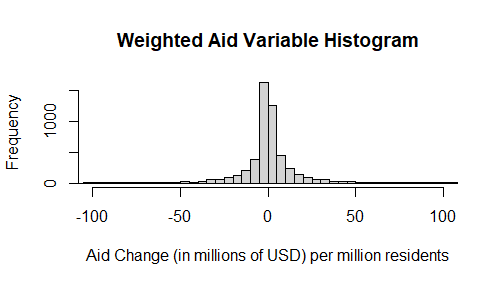
\includegraphics[scale=1]{weightedaidhist}
		\caption{Histogram of Weighted Aid Variable. The x-axis range excludes some outlier points, but those do not affect the overall shape of the distribution}
		\label{fig:weightedaidhist}
	\end{figure}
	
	To measure the urban-rural divide, I include mean travel time in minutes to the nearest city for each subdivision-year, measured in the year 2000 \cite{citytime2000} and in 2015 \cite{citytime2015}. The reasoning behind this measure is that travel time will, on average, decrease not only with city proximity but also as the general quality of transportation infrastructure and road networks increases. This allows decreasing travel time to serve as a rough indicator of the kind of urban build-up described in the theory. These data are supplemented with yearly country-level data on GDP per capita \cite{wb2022}, measured in hundreds of dollars, and V-Dem scores \cite{vdem2023, pemstein2018v} as state-level controls. This results in a timeframe of 1995 through 2014, though population data is generally only available from 2001 onward. When used as a control variable, subdivision population data is logged due to its large values relative to the rest of the data.
	
	This subnational focus provides an ability to control for many potential confounding influences both in this region and within individual states. A subdivision-year data structure focuses on variation within a given state’s subdivisions over time. This allows this analysis to control for states with varied histories that could impact conflict dynamics. Additionally, a subnational focus avoids the potential confounding influence of the way in which the borders of many African states were frequently externally imposed and strategically drawn by colonizing powers. Beyond these concerns, a focus on Sub-Saharan Africa provides useful variation in terms of both foreign aid receipts and conflict occurrence, type, and intensity. Furthermore, this subnational focus also distinguishes this from prior analyses, many of which aggregated to the country-year level. Descriptive statistics for these variables are shown in Table \ref{descstats}.
	
	\begin{table}
		
		\caption{Summary Statistics}
		\centering
		\begin{tabular}[t]{l|r|r}
			\hline
			& Mean & S.D.\\
			\hline
			Aid & 8413611.5 & 21376619.0\\
			\hline
			Population & 1409615.7 & 2227709.0\\
			\hline
			State Deaths & 1.8 & 24.7\\
			\hline
			Rebel Deaths & 2.8 & 33.6\\
			\hline
			Civilian Deaths & 0.9 & 12.7\\
			\hline
			Total Deaths & 8.3 & 73.1\\
			\hline
			GDPPC & 11.2 & 7.0\\
			\hline
			Travel Time (2000) & 444.5 & 387.0\\
			\hline
			Travel Time (2015) & 306.8 & 484.4\\
			\hline
			Electoral Democracy & 0.3 & 0.1\\
			\hline
			Liberal Democracy & 0.2 & 0.1\\
			\hline
			Participatory Democracy & 0.2 & 0.1\\
			\hline
			Deliberative Democracy & 0.2 & 0.1\\
			\hline
			Egalitarian Democracy & 0.2 & 0.1\\
			\hline
		\end{tabular}
		\label{descstats}
	\end{table}

	
\subsection{Model Choice}

The dependent variable for all models is a count of deaths, either sustained by state forces or rebel forces, in a given incident of violence included in the UCDP’s Georeferenced Event Dataset located within the boundaries of a given subdivision during a given year \cite{sundberg2013introducing}. Both dependent variables are substantially over-dispersed, with variances larger than their means. While a Poisson model would be a standard choice given this count data, this over-dispersion violates a foundational assumption of the Poisson model. Due to this, the following analysis instead uses quasi-Poisson models, as suggested by \citet{gelmanhill}, as this relaxes the standard Poisson assumption that the mean equals the variance.

\section{Results}
\subsection{Quasi-Poisson Models Results}

Tables \ref{yearly2000nopop} through \ref{weighted2015} show the outcomes of the quasi-Poisson regressions. These models are divided into two groups: those using aid change in millions of dollars as their primary independent variable, and those using the weighted aid inflows in millions as their primary independent variable. Each of these groups are further split between models that use the city travel time measurements from the year 2000, and those that use the city travel time measurements from the year 2015. Each group uses state forces deaths, rebel forces deaths, and total deaths (state and rebel forces plus civilians) as separate dependent variables. As data on subdivision population is not available for all years of the timeframe, all models are run models both with and without the population variable. All models include controls for the year and fixed-effects terms for each state, which are omitted from the tables for brevity. Each model includes an interaction between the aid change variable and the city travel time variable.

Tables \ref{yearly2000nopop} and \ref{yearly2000pop} show models using the city travel distances from the year 2000, with yearly change in the amount of lagged development aid committed to a given subdivision in a given year as the primary independent variable. In all three models that exclude the population variable, which include subdivision-year data from the full 1995-2014 timeframe, the interaction term is negative but not significant. Its component variables are generally positive but not significant in most models. The results are broadly similar when the population variable is included, narrowing the timeframe to 2001-2014. The interaction term remains negative but not significant in all models, with its component terms generally positively signed but failing to be significant.



\begin{table}[!htbp] \centering 
	  \caption{Quasi-Poisson Regression Results Using 2000 City Travel Times, No Population Variable} 
	\begin{tabular}{@{\extracolsep{5pt}}lccc} 
		\\[-1.8ex]\hline 
		\hline \\[-1.8ex] 
		& \multicolumn{3}{c}{\textit{Dependent variable:}} \\ 
		\cline{2-4} 
		\\[-1.8ex] & State Deaths & Rebel Deaths & Total Deaths \\ 
		\\[-1.8ex] & (1) & (2) & (3)\\ 
		\hline \\[-1.8ex] 
		Foreign Aid Change (in Millions USD) & $-$0.001 & 0.009 & 0.006 \\ 
		& (0.022) & (0.009) & (0.007) \\ 
		& & & \\ 
		City Travel Time (2000) & $-$0.0001 & 0.0004 & 0.0001 \\ 
		& (0.001) & (0.001) & (0.0003) \\ 
		& & & \\ 
		GDP per capita (in Hundreds USD) & 0.473$^{*}$ & 0.615$^{***}$ & 0.397$^{***}$ \\ 
		& (0.276) & (0.193) & (0.077) \\ 
		& & & \\ 
		Electoral Democracy Index & $-$10.836 & $-$4.369 & $-$5.209 \\ 
		& (20.943) & (14.065) & (6.328) \\ 
		& & & \\ 
		Liberal Democracy Index & $-$54.696$^{*}$ & $-$13.711 & $-$21.647$^{***}$ \\ 
		& (30.904) & (18.119) & (7.928) \\ 
		& & & \\ 
		Participatory Democracy Index & $-$52.854 & $-$18.634 & $-$31.445$^{***}$ \\ 
		& (41.964) & (23.258) & (11.463) \\ 
		& & & \\ 
		Deliberative Democracy Index & 20.296 & 6.290 & 7.707 \\ 
		& (19.631) & (12.515) & (4.839) \\ 
		& & & \\ 
		Egalitarian Democracy Index & 111.851$^{*}$ & 22.593 & 47.879$^{***}$ \\ 
		& (59.915) & (41.332) & (18.001) \\ 
		& & & \\ 
		Year & $-$0.053 & $-$0.036 & $-$0.030 \\ 
		& (0.102) & (0.060) & (0.028) \\ 
		& & & \\ 
		Aid:Travel Interaction & $-$0.00000 & $-$0.00001 & $-$0.00000 \\ 
		& (0.00004) & (0.00002) & (0.00001) \\ 
		& & & \\ 
		Constant & 90.208 & 55.298 & 49.409 \\ 
		& (200.092) & (117.090) & (55.579) \\ 
		& & & \\ 
		\hline \\[-1.8ex] 
		Observations & 6,247 & 6,247 & 6,247 \\ 
		\hline 
		\hline \\[-1.8ex] 
		\textit{Note:}  & \multicolumn{3}{r}{$^{*}$p$<$0.1; $^{**}$p$<$0.05; $^{***}$p$<$0.01} \\ 
	\end{tabular} 
	\label{yearly2000nopop}
\end{table} 


\begin{table}[!htbp] \centering 
	\caption{Quasi-Poisson Regression Results Using 2000 City Travel Times, With Population Variable} 
	\begin{tabular}{@{\extracolsep{5pt}}lccc} 
		\\[-1.8ex]\hline 
		\hline \\[-1.8ex] 
		& \multicolumn{3}{c}{\textit{Dependent variable:}} \\ 
		\cline{2-4} 
		\\[-1.8ex] & State Deaths & Rebel Deaths & Total Deaths \\ 
		\\[-1.8ex] & (1) & (2) & (3)\\ 
		\hline \\[-1.8ex] 
		Foreign Aid Change (in Millions USD) & 0.001 & 0.009 & 0.005 \\ 
		& (0.017) & (0.013) & (0.008) \\ 
		& & & \\ 
		City Travel Time (2000) & 0.001 & 0.001 & 0.001 \\ 
		& (0.001) & (0.001) & (0.0005) \\ 
		& & & \\ 
		GDP per capita (in Hundreds USD) & 0.601 & 0.642$^{*}$ & 0.400$^{***}$ \\ 
		& (0.385) & (0.369) & (0.127) \\ 
		& & & \\ 
		Electoral Democracy Index & 14.508 & $-$18.386 & $-$10.533 \\ 
		& (37.864) & (28.375) & (12.675) \\ 
		& & & \\ 
		Liberal Democracy Index & 4.887 & $-$7.436 & $-$17.204 \\ 
		& (49.906) & (40.422) & (16.848) \\ 
		& & & \\ 
		Participatory Democracy Index & $-$62.100 & $-$33.312 & $-$54.620$^{***}$ \\ 
		& (54.073) & (41.622) & (19.543) \\ 
		& & & \\ 
		Deliberative Democracy Index & $-$12.790 & $-$17.512 & $-$20.525$^{**}$ \\ 
		& (29.871) & (28.699) & (10.444) \\ 
		& & & \\ 
		Egalitarian Democracy Index & 38.623 & 86.372 & 111.366$^{**}$ \\ 
		& (118.215) & (108.877) & (48.231) \\ 
		& & & \\ 
		Year & $-$0.024 & $-$0.006 & $-$0.022 \\ 
		& (0.131) & (0.133) & (0.051) \\ 
		& & & \\ 
		Population & 0.227 & 0.481 & 0.422$^{*}$ \\ 
		& (0.482) & (0.556) & (0.226) \\ 
		& & & \\ 
		Aid:Travel Interaction & $-$0.00000 & $-$0.00001 & $-$0.00001 \\ 
		& (0.00003) & (0.00003) & (0.00002) \\ 
		& & & \\ 
		Constant & 21.995 & $-$13.043 & 26.786 \\ 
		& (256.987) & (260.463) & (101.102) \\ 
		& & & \\ 
		\hline \\[-1.8ex] 
		Observations & 4,904 & 4,904 & 4,904 \\ 
		\hline 
		\hline \\[-1.8ex] 
		\textit{Note:}  & \multicolumn{3}{r}{$^{*}$p$<$0.1; $^{**}$p$<$0.05; $^{***}$p$<$0.01} \\ 
	\end{tabular} 
	\label{yearly2000pop}
\end{table}

\newpage

Tables \ref{yearly2015nopop} and \ref{yearly2015pop} show models using the city travel distances from 2015, again using yearly change in the amount of lagged development aid committed to a given subdivision in a given year as the primary independent variable. In the three models excluding the population variable, the interaction term is negative and not significant. Similarly to the previous set of models, its components tend not to be significant, but do show some variation in the direction of their signs. In the models with the population variable, the interaction term is again always negative but not significant, with its component parts always positive and not significant. 

\begin{table}[!htbp] \centering 
	\caption{Quasi-Poisson Regression Results Using 2015 City Travel Times, No Population Variable} 
	\begin{tabular}{@{\extracolsep{5pt}}lccc} 
	\\[-1.8ex]\hline 
	\hline \\[-1.8ex] 
	& \multicolumn{3}{c}{\textit{Dependent variable:}} \\ 
	\cline{2-4} 
	\\[-1.8ex] & State Deaths & Rebel Deaths & Total Deaths \\ 
	\\[-1.8ex] & (1) & (2) & (3)\\ 
	\hline \\[-1.8ex] 
	Foreign Aid Change (in Millions USD) & $-$0.0004 & 0.006 & 0.004 \\ 
	& (0.016) & (0.006) & (0.004) \\ 
	& & & \\ 
	City Travel Time (2015) & $-$0.001 & 0.0001 & 0.0001 \\ 
	& (0.001) & (0.0005) & (0.0002) \\ 
	& & & \\ 
	GDP per capita (in Hundreds USD) & 0.472$^{*}$ & 0.618$^{***}$ & 0.398$^{***}$ \\ 
	& (0.272) & (0.190) & (0.076) \\ 
	& & & \\ 
	Electoral Democracy Index & $-$10.748 & $-$4.422 & $-$5.258 \\ 
	& (20.668) & (13.866) & (6.312) \\ 
	& & & \\ 
	Liberal Democracy Index & $-$54.693$^{*}$ & $-$13.694 & $-$21.624$^{***}$ \\ 
	& (30.446) & (17.865) & (7.900) \\ 
	& & & \\ 
	Participatory Democracy Index & $-$53.036 & $-$18.501 & $-$31.339$^{***}$ \\ 
	& (41.440) & (22.908) & (11.431) \\ 
	& & & \\ 
	Deliberative Democracy Index & 20.236 & 6.229 & 7.739 \\ 
	& (19.344) & (12.332) & (4.816) \\ 
	& & & \\ 
	Egalitarian Democracy Index & 111.998$^{*}$ & 22.547 & 47.776$^{***}$ \\ 
	& (59.059) & (40.752) & (17.946) \\ 
	& & & \\ 
	Year & $-$0.053 & $-$0.036 & $-$0.030 \\ 
	& (0.100) & (0.059) & (0.028) \\ 
	& & & \\ 
	Aid:Travel Interaction & $-$0.00001 & $-$0.00000 & $-$0.00000 \\ 
	& (0.0001) & (0.00002) & (0.00001) \\ 
	& & & \\ 
	Constant & 90.421 & 56.580 & 49.672 \\ 
	& (196.992) & (115.719) & (55.409) \\ 
	& & & \\ 
	\hline \\[-1.8ex] 
	Observations & 6,247 & 6,247 & 6,247 \\ 
	\hline 
	\hline \\[-1.8ex] 
	\textit{Note:}  & \multicolumn{3}{r}{$^{*}$p$<$0.1; $^{**}$p$<$0.05; $^{***}$p$<$0.01} \\  
	\end{tabular} 
	\label{yearly2015nopop}
\end{table}

\begin{table}[!htbp] \centering 
	\caption{Quasi-Poisson Regression Results Using 2015 City Travel Times, With Population Variable} 
	\begin{tabular}{@{\extracolsep{5pt}}lccc} 
\\[-1.8ex]\hline 
\hline \\[-1.8ex] 
& \multicolumn{3}{c}{\textit{Dependent variable:}} \\ 
\cline{2-4} 
\\[-1.8ex] & State Deaths & Rebel Deaths & Total Deaths \\ 
\\[-1.8ex] & (1) & (2) & (3)\\ 
\hline \\[-1.8ex] 
Foreign Aid Change (in Millions USD) & 0.00002 & 0.006 & 0.003 \\ 
& (0.009) & (0.008) & (0.004) \\ 
& & & \\ 
City Travel Time (2015) & 0.0004 & 0.0003 & 0.001$^{**}$ \\ 
& (0.001) & (0.001) & (0.0003) \\ 
& & & \\ 
GDP per capita (in Hundreds USD) & 0.600 & 0.648$^{*}$ & 0.402$^{***}$ \\ 
& (0.374) & (0.334) & (0.118) \\ 
& & & \\ 
Electoral Democracy Index & 15.026 & $-$18.552 & $-$10.734 \\ 
& (37.260) & (25.555) & (11.775) \\ 
& & & \\ 
Liberal Democracy Index & 4.903 & $-$7.571 & $-$17.273 \\ 
& (48.791) & (36.366) & (15.585) \\ 
& & & \\ 
Participatory Democracy Index & $-$62.793 & $-$33.278 & $-$54.475$^{***}$ \\ 
& (53.350) & (37.500) & (18.175) \\ 
& & & \\ 
Deliberative Democracy Index & $-$12.794 & $-$17.527 & $-$20.563$^{**}$ \\ 
& (28.963) & (25.887) & (9.673) \\ 
& & & \\ 
Egalitarian Democracy Index & 38.591 & 86.562 & 111.627$^{**}$ \\ 
& (115.298) & (98.064) & (44.681) \\ 
& & & \\ 
Year & $-$0.023 & $-$0.0003 & $-$0.021 \\ 
& (0.127) & (0.120) & (0.047) \\ 
& & & \\ 
Population & 0.182 & 0.309 & 0.407$^{**}$ \\ 
& (0.434) & (0.452) & (0.194) \\ 
& & & \\ 
Aid:Travel Interaction & $-$0.00000 & $-$0.00000 & $-$0.00000 \\ 
& (0.00002) & (0.00002) & (0.00001) \\ 
& & & \\ 
Constant & 20.350 & $-$20.720 & 26.489 \\ 
& (248.912) & (235.090) & (93.645) \\ 
& & & \\ 
\hline \\[-1.8ex] 
Observations & 4,904 & 4,904 & 4,904 \\ 
\hline 
\hline \\[-1.8ex] 
\textit{Note:}  & \multicolumn{3}{r}{$^{*}$p$<$0.1; $^{**}$p$<$0.05; $^{***}$p$<$0.01} \\ 
	\end{tabular} 
	\label{yearly2015pop}
\end{table} 

\newpage

Tables \ref{weighted2000} and \ref{weighted2015} show models using the amount of lagged aid change in millions per million residents of the subdivision as a different primary independent variable. As this second primary independent variable uses subdivision population data, these models do not include subdivision population as a control variable. Similarly to the models in Tables 2 and 3, these models never return a significant interaction, though the interaction’s sign is more frequently positive than negative, and its components follow a similar pattern.  

\begin{table}[!htbp] \centering 
	\caption{Quasi-Poisson Regression Results Using 2000 City Travel Times, Weighted Aid IV} 
	\begin{tabular}{@{\extracolsep{5pt}}lccc} 
		\\[-1.8ex]\hline 
		\hline \\[-1.8ex] 
		& \multicolumn{3}{c}{\textit{Dependent variable:}} \\ 
		\cline{2-4} 
		\\[-1.8ex] & State Deaths & Rebel Deaths & Total Deaths \\ 
		\\[-1.8ex] & (1) & (2) & (3)\\ 
		\hline \\[-1.8ex] 
		Aid Change per Million Residents (in Millions USD) & $-$0.0001 & 0.003 & 0.0002 \\ 
		& (0.011) & (0.011) & (0.005) \\ 
		& & & \\ 
		City Travel Time (2000) & 0.0003 & 0.0004 & 0.0001 \\ 
		& (0.001) & (0.001) & (0.0004) \\ 
		& & & \\ 
		GDP per capita (in Hundreds USD) & 0.608$^{*}$ & 0.650$^{**}$ & 0.408$^{***}$ \\ 
		& (0.347) & (0.322) & (0.103) \\ 
		& & & \\ 
		Electoral Democracy Index & 12.567 & $-$19.223 & $-$10.683 \\ 
		& (33.175) & (24.894) & (10.144) \\ 
		& & & \\ 
		Liberal Democracy Index & 4.302 & $-$8.187 & $-$16.359 \\ 
		& (42.891) & (35.340) & (13.285) \\ 
		& & & \\ 
		Participatory Democracy Index & $-$59.613 & $-$33.842 & $-$52.513$^{***}$ \\ 
		& (46.908) & (36.599) & (15.511) \\ 
		& & & \\ 
		Deliberative Democracy Index & $-$12.062 & $-$17.916 & $-$19.539$^{**}$ \\ 
		& (26.809) & (25.070) & (8.514) \\ 
		& & & \\ 
		Egalitarian Democracy Index & 38.616 & 89.508 & 106.486$^{***}$ \\ 
		& (102.336) & (95.086) & (38.246) \\ 
		& & & \\ 
		Year & $-$0.013 & 0.010 & $-$0.004 \\ 
		& (0.116) & (0.116) & (0.041) \\ 
		& & & \\ 
		Aid:Travel Interaction & 0.00000 & $-$0.00000 & 0.00000 \\ 
		& (0.00001) & (0.00001) & (0.00000) \\ 
		& & & \\ 
		Constant & 2.728 & $-$37.100 & $-$2.899 \\ 
		& (228.390) & (227.329) & (81.801) \\ 
		& & & \\ 
		\hline \\[-1.8ex] 
		Observations & 4,904 & 4,904 & 4,904 \\ 
		\hline 
		\hline \\[-1.8ex] 
		\textit{Note:}  & \multicolumn{3}{r}{$^{*}$p$<$0.1; $^{**}$p$<$0.05; $^{***}$p$<$0.01} \\  
	\end{tabular} 
	\label{weighted2000}
\end{table}

\begin{table}[!htbp] \centering 
	\caption{Quasi-Poisson Regression Results Using 2015 City Travel Times, Weighted Aid IV} 
	\begin{tabular}{@{\extracolsep{5pt}}lccc} 
		\\[-1.8ex]\hline 
		\hline \\[-1.8ex] 
		& \multicolumn{3}{c}{\textit{Dependent variable:}} \\ 
		\cline{2-4} 
		\\[-1.8ex] & State Deaths & Rebel Deaths & Total Deaths \\ 
		\\[-1.8ex] & (1) & (2) & (3)\\ 
		\hline \\[-1.8ex] 
		Aid Change per Million Residents (in Millions USD) & 0.001 & 0.002 & 0.0004 \\ 
		& (0.009) & (0.009) & (0.004) \\ 
		& & & \\ 
		City Travel Time (2015) & 0.0003 & 0.0002 & 0.0003 \\ 
		& (0.001) & (0.001) & (0.0002) \\ 
		& & & \\ 
		GDP per capita (in Hundreds USD) & 0.609$^{*}$ & 0.651$^{**}$ & 0.408$^{***}$ \\ 
		& (0.345) & (0.313) & (0.103) \\ 
		& & & \\ 
		Electoral Democracy Index & 13.032 & $-$19.338 & $-$10.434 \\ 
		& (32.989) & (24.174) & (10.173) \\ 
		& & & \\ 
		Liberal Democracy Index & 4.802 & $-$8.268 & $-$15.975 \\ 
		& (43.177) & (34.312) & (13.440) \\ 
		& & & \\ 
		Participatory Democracy Index & $-$59.570 & $-$33.789 & $-$52.314$^{***}$ \\ 
		& (46.853) & (35.543) & (15.600) \\ 
		& & & \\ 
		Deliberative Democracy Index & $-$12.102 & $-$17.940 & $-$19.478$^{**}$ \\ 
		& (26.668) & (24.397) & (8.508) \\ 
		& & & \\ 
		Egalitarian Democracy Index & 37.208 & 89.763 & 105.313$^{***}$ \\ 
		& (102.840) & (92.381) & (38.627) \\ 
		& & & \\ 
		Year & $-$0.014 & 0.010 & $-$0.004 \\ 
		& (0.116) & (0.113) & (0.041) \\ 
		& & & \\ 
		Aid:Travel Interaction & 0.00000 & $-$0.00000 & 0.00000 \\ 
		& (0.00000) & (0.00001) & (0.00000) \\ 
		& & & \\ 
		Constant & 5.117 & $-$36.595 & $-$2.115 \\ 
		& (227.093) & (221.181) & (81.907) \\ 
		& & & \\ 
		\hline \\[-1.8ex] 
		Observations & 4,904 & 4,904 & 4,904 \\ 
		\hline 
		\hline \\[-1.8ex] 
		\textit{Note:}  & \multicolumn{3}{r}{$^{*}$p$<$0.1; $^{**}$p$<$0.05; $^{***}$p$<$0.01} \\ 
	\end{tabular} 
	\label{weighted2015}
\end{table}

\newpage

As the interaction terms are central to my hypotheses, marginal effects plots for selected models are shown below in Figures 3 through 5. Due to the lack of significance for the interaction term in all models, the confidence intervals shown in these plots are unsurprisingly overlapping. The plots consistently show, across model specifications and different primary independent variables, an essentially flat line. Aid changes within a subdivision seem to have no impact on state, rebel, or total casualties. Combined with the overlapping confidence intervals that characterize these figures, these marginal effects plots fail to offer support for either hypothesis.

\begin{figure}
	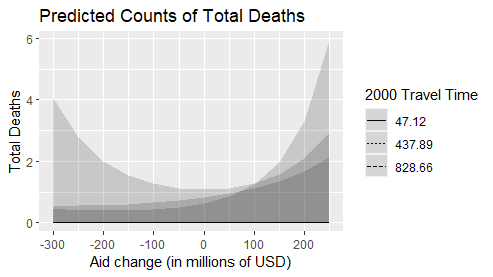
\includegraphics[scale=1]{quasi_pop_tot_00_mfx}
	\caption{Predicted Count of Total Deaths from Table \ref{yearly2000pop}, Model 3. Predictive lines are horizontal and flush with the x-axis.}
\end{figure}

\begin{figure}
	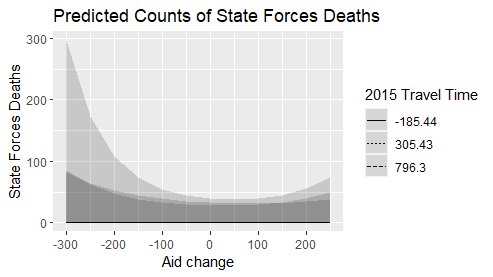
\includegraphics[scale=1]{quasi_pop_a_mfx}
	\caption{Predicted Count of State Forces Deaths from Table \ref{yearly2015pop}, Model 1. Predictive lines are horizontal and flush with the x-axis.}
\end{figure}

\begin{figure}
	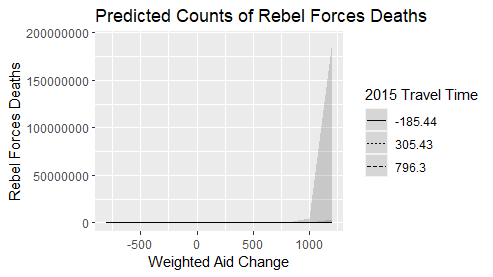
\includegraphics[scale=1]{weighted_b_15_mfx}
	\caption{Predicted Count of Rebel Forces Deaths from Table \ref{weighted2015}, Model 2. Predictive lines are horizontal and flush with the x-axis.}
\end{figure}

\subsection{Robustness Checks}

There may be some concern that these results are impacted by multicollinearity amongst some of the predictor variables. Variance inflation factor (VIF) scores for the GDP per capita and V-Dem variables show them to be strongly correlated in all models, with massive VIF scores in all models shown in the tables above. As a robustness check, Tables \ref{robustyearly2000nopop} through X in the appendix show the results of running all models again, dropping the V-Dem variables. The direction and lack of significance of the interaction term never changes. This suggests that the lack of findings in the main models is not wholly driven by this collinearity.

\section{Discussion}

While these results do not provide substantial support for either hypothesis, the results themselves are still worthy of consideration. The lack of significance for the interaction term may not necessarily indicate the absence of these commitment problems from civil wars at the subnational level. Alternatively, these results could be caused by inflows of aid simultaneously increasing the capabilities of one side in an area while decreasing the capabilities of the opposing side, with these two effects cancelling each other out in the aggregate. While this analysis attempts to control for this by using deaths from both state forces and rebel groups as separate dependent variables, in order to try to isolate the effects of these changes on a single side of the conflict, there is no guarantee that this method was always effective. 

As an additional consideration, these results are also necessarily bounded by the limits of Aiddata itself as a source. While incredibly useful for its subnational disaggregation of aid, this dataset has some limitations in its yearly range of coverage, such as aid data only being recorded from 1995 through 2014. This necessarily limits the timeframe which can be investigated, and the possibility remains that a wider timeframe might have produced stronger results. 

Despite these limitations, these results still suggest some directions for future research efforts. One potential direction is to consider other types of aid, such as military aid, or humanitarian aid in the wake of natural disasters. As this paper focuses on one specific type of aid, investigations into other types could prove useful. Some work has already investigated American counterinsurgency aid \cite{berman2013modest, sexton2016aid}, but if a subnational analysis of the effects of some other types of aid could be conducted, that could provide additional insight into its effects. Another possibility is that these theorized commitment problems, at least as they pertain to foreign aid, are either too rare or complicated to be easily modeled. If this is the case, a more qualitative method of investigation focusing on specific cases and time periods could be more fruitful in uncovering cases where commitment problems occur in ways congruent with the theory. Conversely, if such qualitative case studies did not uncover such evidence, this would still be useful for future theory development. 

Regardless of the results of future research, this paper still contributes to the study of conflict processes through its puzzling findings. The lack of initial empirical support for the hypothesized commitment problems increasing the level of violence of civil wars in Sub-Saharan Africa is disappointing. However, while unexpected, these results still ultimately provide directions for numerous potential future research projects.	

	
	%===================References=====================
	\newpage
	\bibliographystyle{apsr}
	\bibliography{draft6.bib}
\newpage

\section{Appendix}

\subsection{Regressions Excluding V-Dem Variables}

\begin{table}[!htbp] \centering 
	\caption{Quasi-Poisson Regression Results Using 2000 City Travel Times, No Population Variable, Excluding V-Dem } 
	\label{robustyearly2000nopop} 
	\begin{tabular}{@{\extracolsep{5pt}}lccc} 
		\\[-1.8ex]\hline 
		\hline \\[-1.8ex] 
		& \multicolumn{3}{c}{\textit{Dependent variable:}} \\ 
		\cline{2-4} 
		\\[-1.8ex] & State Deaths & Rebel Deaths & Total Deaths \\ 
		\\[-1.8ex] & (1) & (2) & (3)\\ 
		\hline \\[-1.8ex] 
		Foreign Aid Change (in Millions USD) & 0.0004 & 0.009 & 0.005 \\ 
		& (0.008) & (0.006) & (0.006) \\ 
		& & & \\ 
		City Travel Time (2000) & $-$0.0001 & 0.0004 & 0.0001 \\ 
		& (0.0004) & (0.0004) & (0.0003) \\ 
		& & & \\ 
		GDP per capita (in Hundreds USD) & 0.161$^{**}$ & 0.515$^{***}$ & 0.310$^{***}$ \\ 
		& (0.066) & (0.101) & (0.058) \\ 
		& & & \\ 
		Year & $-$0.133$^{***}$ & $-$0.093$^{***}$ & $-$0.109$^{***}$ \\ 
		& (0.028) & (0.031) & (0.021) \\ 
		& & & \\ 
		Aid:Travel Interaction & $-$0.00000 & $-$0.00001 & $-$0.00000 \\ 
		& (0.00001) & (0.00001) & (0.00001) \\ 
		& & & \\ 
		Constant & 261.503$^{***}$ & 172.004$^{***}$ & 210.611$^{***}$ \\ 
		& (54.716) & (59.764) & (42.048) \\ 
		& & & \\ 
		\hline \\[-1.8ex] 
		Observations & 6,247 & 6,247 & 6,247 \\ 
		\hline 
		\hline \\[-1.8ex] 
		\textit{Note:}  & \multicolumn{3}{r}{$^{*}$p$<$0.1; $^{**}$p$<$0.05; $^{***}$p$<$0.01} \\ 
	\end{tabular} 
\end{table} 

\begin{table}[!htbp] \centering 
	\caption{Quasi-Poisson Regression Results Using 2000 City Travel Times, With Population Variable, Excluding V-Dem } 
	\label{robustyearly2000pop} 
	\begin{tabular}{@{\extracolsep{5pt}}lccc} 
		\\[-1.8ex]\hline 
		\hline \\[-1.8ex] 
		& \multicolumn{3}{c}{\textit{Dependent variable:}} \\ 
		\cline{2-4} 
		\\[-1.8ex] & State Deaths & Rebel Deaths & Total Deaths \\ 
		\\[-1.8ex] & (1) & (2) & (3)\\ 
		\hline \\[-1.8ex] 
		Foreign Aid Change (in Millions USD) & 0.001 & 0.010 & 0.006 \\ 
		& (0.008) & (0.012) & (0.006) \\ 
		& & & \\ 
		City Travel Time (2000) & 0.001 & 0.001 & 0.001$^{*}$ \\ 
		& (0.0005) & (0.001) & (0.0004) \\ 
		& & & \\ 
		GDP per capita (in Hundreds USD) & 0.644$^{***}$ & 0.621$^{**}$ & 0.449$^{***}$ \\ 
		& (0.178) & (0.290) & (0.099) \\ 
		& & & \\ 
		Year & $-$0.079 & $-$0.076 & $-$0.107$^{***}$ \\ 
		& (0.052) & (0.099) & (0.037) \\ 
		& & & \\ 
		Population & 0.244 & 0.498 & 0.434$^{**}$ \\ 
		& (0.225) & (0.527) & (0.190) \\ 
		& & & \\ 
		Aid:Travel Interaction & $-$0.00000 & $-$0.00001 & $-$0.00001 \\ 
		& (0.00002) & (0.00003) & (0.00001) \\ 
		& & & \\ 
		Constant & 133.342 & 128.234 & 195.451$^{***}$ \\ 
		& (101.450) & (194.286) & (72.452) \\ 
		& & & \\ 
		\hline \\[-1.8ex] 
		Observations & 4,904 & 4,904 & 4,904 \\ 
		\hline 
		\hline \\[-1.8ex] 
		\textit{Note:}  & \multicolumn{3}{r}{$^{*}$p$<$0.1; $^{**}$p$<$0.05; $^{***}$p$<$0.01} \\ 
	\end{tabular} 
\end{table} 

\begin{table}[!htbp] \centering 
	\caption{Quasi-Poisson Regression Results Using 2015 City Travel Times, No Population Variable, Excluding V-Dem } 
	\label{robustyearly2015nopop} 
	\begin{tabular}{@{\extracolsep{5pt}}lccc} 
		\\[-1.8ex]\hline 
		\hline \\[-1.8ex] 
		& \multicolumn{3}{c}{\textit{Dependent variable:}} \\ 
		\cline{2-4} 
		\\[-1.8ex] & State Deaths & Rebel Deaths & Total Deaths \\ 
		\\[-1.8ex] & (1) & (2) & (3)\\ 
		\hline \\[-1.8ex] 
		Foreign Aid Change (in Millions USD) & 0.001 & 0.007$^{*}$ & 0.005 \\ 
		& (0.006) & (0.004) & (0.004) \\ 
		& & & \\ 
		City Travel Time (2015) & $-$0.001$^{*}$ & 0.0001 & 0.0001 \\ 
		& (0.0003) & (0.0003) & (0.0002) \\ 
		& & & \\ 
		GDP per capita (in Hundreds USD) & 0.160$^{**}$ & 0.517$^{***}$ & 0.310$^{***}$ \\ 
		& (0.067) & (0.099) & (0.058) \\ 
		& & & \\ 
		Year & $-$0.134$^{***}$ & $-$0.094$^{***}$ & $-$0.109$^{***}$ \\ 
		& (0.028) & (0.030) & (0.021) \\ 
		& & & \\ 
		Aid:Travel Interaction & $-$0.00001 & $-$0.00000 & $-$0.00000 \\ 
		& (0.00002) & (0.00001) & (0.00001) \\ 
		& & & \\ 
		Constant & 261.834$^{***}$ & 173.384$^{***}$ & 210.846$^{***}$ \\ 
		& (54.855) & (59.181) & (42.020) \\ 
		& & & \\ 
		\hline \\[-1.8ex] 
		Observations & 6,247 & 6,247 & 6,247 \\ 
		\hline 
		\hline \\[-1.8ex] 
		\textit{Note:}  & \multicolumn{3}{r}{$^{*}$p$<$0.1; $^{**}$p$<$0.05; $^{***}$p$<$0.01} \\ 
	\end{tabular} 
\end{table} 

\begin{table}[!htbp] \centering 
	\caption{Quasi-Poisson Regression Results Using 2015 City Travel Times, With Population Variable, Excluding V-Dem } 
	\label{robustyearly2015pop} 
	\begin{tabular}{@{\extracolsep{5pt}}lccc} 
		\\[-1.8ex]\hline 
		\hline \\[-1.8ex] 
		& \multicolumn{3}{c}{\textit{Dependent variable:}} \\ 
		\cline{2-4} 
		\\[-1.8ex] & State Deaths & Rebel Deaths & Total Deaths \\ 
		\\[-1.8ex] & (1) & (2) & (3)\\ 
		\hline \\[-1.8ex] 
		Foreign Aid Change (in Millions USD) & 0.0001 & 0.006 & 0.003 \\ 
		& (0.004) & (0.007) & (0.003) \\ 
		& & & \\ 
		City Travel Time (2015) & 0.0004 & 0.0003 & 0.001$^{***}$ \\ 
		& (0.0003) & (0.001) & (0.0002) \\ 
		& & & \\ 
		GDP per capita (in Hundreds USD) & 0.645$^{***}$ & 0.624$^{**}$ & 0.450$^{***}$ \\ 
		& (0.173) & (0.260) & (0.094) \\ 
		& & & \\ 
		Year & $-$0.077 & $-$0.071 & $-$0.106$^{***}$ \\ 
		& (0.050) & (0.089) & (0.035) \\ 
		& & & \\ 
		Population & 0.195 & 0.319 & 0.416$^{**}$ \\ 
		& (0.203) & (0.425) & (0.166) \\ 
		& & & \\ 
		Aid:Travel Interaction & $-$0.00000 & $-$0.00001 & $-$0.00000 \\ 
		& (0.00001) & (0.00002) & (0.00001) \\ 
		& & & \\ 
		Constant & 131.031 & 120.816 & 195.387$^{***}$ \\ 
		& (98.541) & (173.792) & (68.634) \\ 
		& & & \\ 
		\hline \\[-1.8ex] 
		Observations & 4,904 & 4,904 & 4,904 \\ 
		\hline 
		\hline \\[-1.8ex] 
		\textit{Note:}  & \multicolumn{3}{r}{$^{*}$p$<$0.1; $^{**}$p$<$0.05; $^{***}$p$<$0.01} \\ 
	\end{tabular} 
\end{table}

\begin{table}[!htbp] \centering 
	\caption{Quasi-Poisson Regression Results Using 2000 City Travel Times, Weighted Aid IV, No V-Dem Variables} 
	\label{robustweighted2000} 
	\begin{tabular}{@{\extracolsep{5pt}}lccc} 
		\\[-1.8ex]\hline 
		\hline \\[-1.8ex] 
		& \multicolumn{3}{c}{\textit{Dependent variable:}} \\ 
		\cline{2-4} 
		\\[-1.8ex] & State Deaths & Rebel Deaths & Total Deaths \\ 
		\\[-1.8ex] & (1) & (2) & (3)\\ 
		\hline \\[-1.8ex] 
		Aid Change per Million Residents (in Millions USD) & 0.00004 & 0.003 & $-$0.0002 \\ 
		& (0.006) & (0.010) & (0.004) \\ 
		& & & \\ 
		City Travel Time (2000) & 0.0003 & 0.0004 & 0.0001 \\ 
		& (0.0004) & (0.001) & (0.0003) \\ 
		& & & \\ 
		GDP per capita (in Hundreds USD) & 0.648$^{***}$ & 0.629$^{**}$ & 0.451$^{***}$ \\ 
		& (0.178) & (0.256) & (0.093) \\ 
		& & & \\ 
		Year & $-$0.069 & $-$0.061 & $-$0.089$^{***}$ \\ 
		& (0.051) & (0.087) & (0.034) \\ 
		& & & \\ 
		Aid:Travel Interaction & 0.00000 & $-$0.00000 & 0.00000 \\ 
		& (0.00000) & (0.00001) & (0.00000) \\ 
		& & & \\ 
		Constant & 117.527 & 105.025 & 166.537$^{**}$ \\ 
		& (100.050) & (170.313) & (67.335) \\ 
		& & & \\ 
		\hline \\[-1.8ex] 
		Observations & 4,904 & 4,904 & 4,904 \\ 
		\hline 
		\hline \\[-1.8ex] 
		\textit{Note:}  & \multicolumn{3}{r}{$^{*}$p$<$0.1; $^{**}$p$<$0.05; $^{***}$p$<$0.01} \\ 
	\end{tabular} 
\end{table} 

\begin{table}[!htbp] \centering 
	\caption{Quasi-Poisson Regression Results Using 2000 City Travel Times, Weighted Aid IV, No V-Dem Variables} 
	\label{robustweighted2015} 
	\begin{tabular}{@{\extracolsep{5pt}}lccc} 
		\\[-1.8ex]\hline 
		\hline \\[-1.8ex] 
		& \multicolumn{3}{c}{\textit{Dependent variable:}} \\ 
		\cline{2-4} 
		\\[-1.8ex] & State Deaths & Rebel Deaths & Total Deaths \\ 
		\\[-1.8ex] & (1) & (2) & (3)\\ 
		\hline \\[-1.8ex] 
		Aid Change per Million Residents (in Millions USD) & 0.001 & 0.002 & $-$0.0001 \\ 
		& (0.004) & (0.008) & (0.003) \\ 
		& & & \\ 
		City Travel Time (2000) & 0.0003 & 0.0002 & 0.0003 \\ 
		& (0.0003) & (0.001) & (0.0002) \\ 
		& & & \\ 
		GDP per capita (in Hundreds USD) & 0.649$^{***}$ & 0.629$^{**}$ & 0.452$^{***}$ \\ 
		& (0.176) & (0.249) & (0.093) \\ 
		& & & \\ 
		Year & $-$0.070 & $-$0.061 & $-$0.090$^{***}$ \\ 
		& (0.051) & (0.084) & (0.034) \\ 
		& & & \\ 
		Population & 0.00000 & $-$0.00000 & 0.00000 \\ 
		& (0.00000) & (0.00001) & (0.00000) \\ 
		& & & \\ 
		Aid:Travel Interaction & 118.689 & 105.299 & 167.551$^{**}$ \\ 
		& (99.071) & (165.660) & (67.095) \\ 
		& & & \\ 
		\hline \\[-1.8ex] 
		Observations & 4,904 & 4,904 & 4,904 \\ 
		\hline 
		\hline \\[-1.8ex] 
		\textit{Note:}  & \multicolumn{3}{r}{$^{*}$p$<$0.1; $^{**}$p$<$0.05; $^{***}$p$<$0.01} \\ 
	\end{tabular} 
\end{table} 

\subsection{Regressions with Democratic and Autocratic Sub-samples}

The following models repeat the main analysis after dividing the data into democratic and autocratic sub-samples. This is accomplished through V-Dem’s Regimes of the World measure, which is an ordinal measure dividing regimes into one of four categories: closed autocracy, electoral autocracy, electoral democracy, or liberal democracy \cite{vdemcodebook, luhrmann2018regimes}. Autocratic subdivision-years substantially outnumbered democratic ones, with 6663 autocratic observations to 997 democratic ones.





	%===================End Document===================
\end{document}